\documentclass[conference]{IEEEtran}
\IEEEoverridecommandlockouts
\usepackage{cite}
\usepackage{amsmath,amssymb,amsfonts}
\usepackage{algorithmic}
\usepackage{graphicx}
\usepackage{textcomp}
\usepackage{xcolor}
\usepackage{booktabs}
\usepackage{array}
\usepackage{url}
\usepackage[hidelinks]{hyperref}
\def\BibTeX{{\rm B\kern-.05em{\sc i\kern-.025em b}\kern-.08em
    T\kern-.1667em\lower.7ex\hbox{E}\kern-.125emX}}

\newcommand{\ci}[2]{{\scriptsize[#1,\,#2]}}
\newcommand{\absrel}{AbsRel}
\newcommand{\dOne}{$\delta_1$}
\newcommand{\gt}{g}
\newcommand{\pred}{\hat{d}}
\newcommand{\n}[1]{{\scriptsize($n$=#1)}}
\graphicspath{{figs/}}
\renewcommand{\topfraction}{0.95}
\renewcommand{\bottomfraction}{0.6}
\renewcommand{\textfraction}{0.05}
\renewcommand{\floatpagefraction}{0.85}
\renewcommand{\dbltopfraction}{0.95}
\renewcommand{\dblfloatpagefraction}{0.85}
\setcounter{topnumber}{3}
\setcounter{dbltopnumber}{2}
\setcounter{totalnumber}{5}

\begin{document}

\title{How Well Do Zero-Shot Depth Anything Models Work Off-Road? A LiDAR Evaluation of DA2 and DA3 on RELLIS-3D}

\author{\IEEEauthorblockN{Author Name}
\IEEEauthorblockA{\textit{Department} \\
\textit{Organization}\\
City, Country \\
email@example.com}
}

\maketitle

\begin{abstract}
Monocular depth models like Depth Anything are starting to be used on off-road robots without any extra training. A recent open-source off-road navigation stack does exactly this with Depth Anything V2 and a Sobel edge mask to throw away unreliable pixels. In this paper we test how well this actually works on real off-road data. We evaluate four zero-shot models (Depth Anything V2 Small and Base, and Depth Anything 3 Small and Base) on 830 frames from a held-out sequence of RELLIS-3D, using projected LiDAR as ground truth and the LiDAR semantic labels to split the errors by terrain type and distance. We froze the evaluation protocol before looking at any test number, and we report 95 percent block-bootstrap intervals for everything. We found four things. DA3-Small is more accurate than both DA2 models when both are aligned the same way (0.030 lower AbsRel overall, 0.108 lower on depth edges), but on grass the models are about the same. All four models compress far range: between 49 and 70 percent of vegetation points beyond 20 m are predicted closer than 0.8 times the LiDAR depth, and no per-image scale or scale-and-shift fit removes this. The confidence output of DA3 is a good detector of its own errors (AUROC 0.88 to 0.92). And at the same pixel budget, removing pixels by low confidence lowers AbsRel much more than removing them by Sobel edge strength (0.100 against 0.151 at a 20 percent budget), while the Sobel signal itself is barely better than random. We also report a small camera-LiDAR calibration offset in the dataset and show which results change because of it. The projection and evaluation code is released.
\end{abstract}

\begin{IEEEkeywords}
monocular depth estimation, off-road robotics, depth foundation models, uncertainty, LiDAR, RELLIS-3D
\end{IEEEkeywords}

\section{Introduction}
Depth Anything V2 (DA2)~\cite{da2} and Depth Anything 3 (DA3)~\cite{da3} give dense relative depth from a single image and need no training on the target scene. This makes them interesting for off-road robots, because LiDAR is expensive and heavy and there is very little labelled depth data for off-road terrain. The open-source off-road stack of Marsal et al.~\cite{offroadnav} uses zero-shot DA2 as its camera depth source and mentions the lack of fine-tuning as an advantage. To remove unreliable pixels it runs a Sobel edge detector over the disparity map and masks out everything near an edge, because monocular depth is usually worst at depth discontinuities.

The same paper also reports a problem. In a simulated scene with tall grass, DA2 gave blurry depth and outlier 3D points behind real obstacles. The edge mask did not catch them and the planner saw obstacles that were not there. This made us ask two questions. First, how big are the errors of these models on real off-road scenes, and where are they: in grass, in trees, at edges, or far away? Second, DA3 has a per-pixel confidence output that DA2 does not have. Does that confidence point to the pixels that are actually wrong, and is it better than the edge mask?

To answer this we built a LiDAR-based evaluation on RELLIS-3D~\cite{rellis}, which has a 64-beam Ouster LiDAR, a 1920$\times$1200 camera and point-wise semantic labels. We project the LiDAR into the camera at the resolution the models run at, remove occluded points, and score DA2-Small, DA2-Base, DA3-Small and DA3-Base on 830 frames of a sequence that was not used for any decision about the protocol. The protocol itself (test sequence, alignment method, edge band, bootstrap settings) was committed to version control before we computed any test number.

The contributions of this paper are:
\begin{enumerate}
\item A zero-shot evaluation of DA2 and DA3 on real off-road LiDAR, split by terrain class and distance, with paired comparisons at equal alignment and bootstrap intervals (Sec.~\ref{sec:acc}--\ref{sec:dist}).
\item Evidence that all four models compress far range: far vegetation is predicted too close and near vegetation too far, and per-image alignment does not fix it (Sec.~\ref{sec:dist}). We think this is the real-data version of the phantom obstacle problem.
\item An evaluation of DA3's confidence as an error detector (Sec.~\ref{sec:conf}) and a comparison against the Sobel mask of~\cite{offroadnav} at equal pixel budgets (Sec.~\ref{sec:filter}). Confidence wins at every budget.
\item A LiDAR projection and evaluation pipeline with built-in sanity checks, plus a sensitivity analysis for a calibration offset we found in the dataset (Sec.~\ref{sec:gt}, \ref{sec:sens}). The code is released under Apache~2.0.
\end{enumerate}

Everything was run on one laptop with an 8\,GB GPU. We do not fine-tune anything in this paper. Whether a small fine-tune on RELLIS-3D fixes the compression is the follow-up question, and the numbers here are the baseline for it.

\section{Related Work}
\textbf{Depth foundation models.} Depth Anything~\cite{da1} and DA2~\cite{da2} use a DINOv2 encoder and a DPT head trained on large amounts of unlabelled images, and predict affine-invariant inverse depth. DA3~\cite{da3} uses a single transformer that predicts depth up to scale, and also outputs a per-pixel confidence trained with a confidence-weighted L1 loss, so low confidence should mean high expected error. The model cards list 0.08B parameters for DA3-Small and 0.12B for DA3-Base\footnote{The DA3 paper tables say 0.03B and 0.11B. We use the model card numbers.}. As far as we know, neither family has been evaluated against LiDAR on off-road vegetation.

\textbf{Off-road perception.} RELLIS-3D~\cite{rellis} provides synchronised camera, LiDAR and semantic labels from a rural campus. Its calibration was revised in v1.1, and the project's issue tracker still has reports of image--LiDAR mismatch. The stack of~\cite{offroadnav} combines a LiDAR branch and a monocular branch based on zero-shot DA2 with an edge mask. It reports successful real-world tests on flat terrain and the tall-grass problem in simulation. Our evaluation targets that problem on real data.

\textbf{Confidence of 3D foundation models.} Several recent papers look at the built-in confidence of feed-forward 3D models other than DA3: VGGT on DTU~\cite{hillemann}, a calibration audit of several reconstruction models~\cite{deng}, and evidential or perturbation-based alternatives~\cite{trust3r,revar3r}. The general finding is that the native confidence ranks errors reasonably well but is overconfident. Landgraf et al.~\cite{landgraf} review uncertainty for depth foundation models, mostly indoors. We use the same ranking-based tools (sparsification curves and AUSE~\cite{ilg}, plus AUROC) on DA3 outdoors.

\textbf{Fine-tuning Depth Anything.} Fine-tuning Depth Anything for a new domain is common (underwater~\cite{underwater}, endoscopy~\cite{endo}, canopy height~\cite{canopy}). We did not find any work that does this on RELLIS-3D or evaluates DA3 confidence on off-road LiDAR, but our search was limited.

\section{Ground Truth from LiDAR}\label{sec:gt}

\subsection{Projection and occlusion filter}
RELLIS-3D gives a per-sequence camera-to-LiDAR transform, intrinsics and a distortion vector (the distortion only appears in the official projection notebook). We invert the transform to bring the Ouster points into the camera frame, keep points with $z>0$, and drop points beyond $1.2\times$ the half field of view before applying distortion, since the polynomial can fold those back into the image. Points are projected directly at the models' input resolution of $504\times322$ by scaling the intrinsics (with the half-pixel offset $(u+0.5)\,s-0.5$), with a z-buffer so the nearest point wins. We never resize a depth map by interpolation.

Sparse LiDAR projected into an image lets background points show through foreground edges. To handle this, we look at a $\pm4$\,px window covering the pixel's row and the rows above it, and drop a point if it is farther than the nearest point in the window by more than 20\% and 0.5\,m. Only looking at the rows above means distant ground is not wrongly removed. The filter keeps 94.5--98.2\% of points per sequence.

\subsection{Sanity checks}
A projection with the wrong transform direction or the wrong scan still looks plausible, so we checked it with a metric that does not involve any depth model: how often the LiDAR point label agrees with the 2D image annotation at the projected pixel. With the correct projection the median agreement is 0.77--0.91 per sequence. Not inverting the transform drops it to 0.09--0.28, and pairing with a scan one second later lowers it in every sequence. Distortion on or off makes no measurable difference, so we use the official values.

\subsection{A residual calibration offset}\label{sec:calib}
Even with the correct projection, LiDAR points land a few pixels too high. A full-resolution crop of sequence 00001 shows the top LiDAR ring floating 12--15 source pixels (3--4\,px at our resolution) above a barrier, which matches a rotation error of about $0.3^\circ$. Shifting the projected labels vertically gives the best agreement at $+5$ to $+6$\,px in every sequence. We fitted a per-sequence pixel offset on classes with sharp boundaries (pole, vehicle, fence, concrete, barrier), using labels only. With an acceptance rule fixed before fitting, two sequences gave stable estimates and three did not, including the test sequence. We do not know the cause. Sequences that share one extrinsics file give different estimates, so it could be per-frame pitch or timing. It matters because 4\,px on ground at 20\,m is about 9\% depth error.

So we use the official calibration as the main ground truth and also recompute every result against a second ``sensitivity'' ground truth built from the five offset estimates. Sec.~\ref{sec:sens} says which results change.

\section{Evaluation Protocol}\label{sec:protocol}
Everything below was frozen in version control before any test number was computed. The evaluation script refuses to run on the test split unless the frozen flag is set and the working tree is clean.

\subsection{Valid pixels and alignment}
Valid pixels are occlusion-filtered LiDAR pixels with depth between 1 and 80\,m. This set only depends on the ground truth, so every model is scored on the same pixels. Each image needs at least 200 valid pixels; none fell below.

Predictions are aligned to the ground truth once per image on all valid pixels, and that alignment is then used for every subset. The two model families output different things, so each has its own primary method, and we report the others as a fairness check:
\begin{itemize}
\item DA3 (depth up to scale). Primary: \texttt{median}, scale only, $s=\operatorname{median}(\gt/\pred)$. Also \texttt{ls} and \texttt{huber}: scale and shift in inverse depth.
\item DA2 (relative disparity). Primary: \texttt{ls}, scale and shift in disparity against $1/\gt$, then inverted to depth. Also \texttt{huber}.
\end{itemize}
Huber uses iteratively reweighted least squares with $\delta=1.345\,\hat\sigma$ and $\hat\sigma=1.4826\cdot\mathrm{MAD}$~\cite{huber}; these are the textbook values. After alignment, depth is clamped to $[1,80]$\,m. Less than 0.2\% of valid pixels are clamped for DA3 and less than 0.7\% for DA2. One limitation to keep in mind: per-image alignment uses ground truth that a robot would not have.

\subsection{Metrics and subsets}
For each image we compute \absrel{}, RMSE (m), \dOne{} (share of pixels with $\max(\pred/\gt,\gt/\pred)<1.25$), the \emph{phantom rate} (share with $\pred<0.8\,\gt$, i.e.\ free space predicted too close) and the \emph{overshoot rate} ($\pred>1.25\,\gt$). We then average over images. Phantom rate is only compared within one alignment, because median scaling puts about half the pixels below ratio 1 by construction.

Subsets come from the LiDAR point labels, merged into groups: \emph{grass}; \emph{trees/bushes} (tree, bush); \emph{ground} (dirt, mud, asphalt, concrete); \emph{other}; and \emph{vegetation} (grass plus trees/bushes). Distance bins are 0--10, 10--20 and 20--80\,m, which hold 62\%, 29\% and 9\% of validation points. If a subset has fewer than 50 pixels in an image, that image is skipped for that subset, and we write the number of images used as $(n{=}\cdot)$ when it is below 90\% of 830.

A pixel is in the \emph{edge band} if some in-range LiDAR point within row $\pm1$ and column $\pm4$ lies across a depth jump of ratio $>1.2$ (\emph{edge\_depth}) or across a boundary between groups (\emph{edge\_semantic}). \emph{edge} is the union. Row $\pm1$ never reaches the next LiDAR ring (about 7 rows away), so flat ground is not flagged, but horizontal edges between rings are also missed.

\subsection{Confidence (DA3 only)}
DA3 outputs $\mathrm{conf}=\exp(x)+1\ge1$. Per image we compute the AUROC of $-\mathrm{conf}$ for detecting pixels with \absrel{} $>0.25$ after alignment (images with fewer than 20 positives or negatives are skipped; that is 0--1 of 830). For sparsification we recompute \absrel{} after removing the lowest-confidence $0,5,\dots,95\%$ of valid pixels, with ties broken randomly and without refitting the alignment. AUSE is the area between the confidence curve and the oracle curve (removal by true error). AURG is the area gained over random removal, which we also report because AUSE scales with the base error. Both only depend on the ranking of the confidence values, so we never assume the confidence is calibrated.

\subsection{Filtering comparison}\label{sec:filterproto}
We re-implemented the edge mask of~\cite{offroadnav} from its code: min--max scale the disparity to 8 bits, $5\times5$ Gaussian blur, Sobel with kernel 3, magnitude by \texttt{hypot}, scale by the maximum, Otsu threshold~\cite{otsu} per image, and dilate with an elliptical kernel whose diameter is the ``thickness''. Note that the threshold is Otsu, not fixed, the 5\,px thickness is a diameter (about $\pm2$\,px), and the shipped default is actually Canny with thickness 10. The input is disparity for DA2 and inverse depth for DA3.

The primary comparison removes a fixed share of 10, 20, 30 or 50\% of the valid pixels per image. \emph{Sobel-ranked} removes the pixels with the highest dilated Sobel magnitude, \emph{confidence-ranked} removes the lowest DA3 confidence, and \emph{random} removes at random (10 seeds). A secondary comparison applies the faithful Otsu mask at thickness 3, 5 and 9 and compares it with confidence removal matched to the same number of valid pixels (\emph{conf\_valid}) or the same share of the whole image (\emph{conf\_all}). We made the fixed-budget version primary before the freeze because on validation the Otsu mask removed 73--86\% of valid pixels, which leaves too few pixels for a fair comparison at its own budget.

\subsection{Statistics}
All metrics are per image. We report means with 95\% percentile intervals from a block bootstrap (1{,}000 resamples, seed 0, blocks of 30 consecutive evaluated frames, about 15\,s of driving). We picked 30 on validation, where per-image \absrel{} stayed autocorrelated up to lag 20--30 for DA2. Paired differences are against DA3-Small, over images valid for both models, with the same alignment on both sides.

\section{Experimental Setup}

\subsection{Models}\label{sec:models}
Table~\ref{tab:models} lists the four models. DA3 runs as upstream (bf16 backbone, fp32 head). DA2 runs in fp32 because bf16 quantised its disparity by about 0.4\%. All models get $504\times322$ inputs: resizing the long side to 504 gives $504\times315$, which the DA3 pipeline rounds up to a multiple of 14. Latency is the median of 30 runs after 5 warm-up runs. Since the precisions differ, it is not a fair speed comparison. Everything ran on a laptop (i7-13620H, 16\,GB RAM, RTX~4060 Laptop 8\,GB) under WSL2 with PyTorch 2.11; the DA3 repository was at commit \texttt{3d835ec} (checkpoints \texttt{DA3-SMALL}, \texttt{DA3-BASE}) and DA2 came from the Hugging Face \texttt{-hf} checkpoints. Seeds are fixed everywhere.

\begin{table}[!t]
\caption{Zero-shot models and inference cost at $504\times322$.}
\label{tab:models}
\centering
\small
\begin{tabular}{lcccrr}
\toprule
Model & Params & Output & Conf. & VRAM & Latency \\
\midrule
DA3-S & 0.08B & depth$^a$ & yes & 285\,MB & 25.3\,ms \\
DA3-B & 0.12B & depth$^a$ & yes & 896\,MB & 43.3\,ms \\
DA2-S & 24.8M & disparity$^b$ & no & 170\,MB & 14.5\,ms \\
DA2-B & 97.5M & disparity$^b$ & no & 490\,MB & 34.7\,ms \\
\bottomrule
\multicolumn{6}{l}{\scriptsize $^a$up to scale; $^b$relative (affine-invariant). DA3 bf16/fp32, DA2 fp32.}
\end{tabular}
\end{table}

\subsection{Dataset and split}
RELLIS-3D has five sequences and 13{,}556 frames, each image matched to an Ouster scan by frame number. 6{,}234 frames have 2D image annotations, and all scans have point labels. The licence is CC~BY-NC-SA~3.0. Table~\ref{tab:split} shows the class mix per sequence.

We fixed the split before looking at any model accuracy. Sequence 00002 is the test sequence because it has the most grass and vegetation pixels. 00001 is validation because its class mix is closest to test. 00000, 00003 and 00004 are kept for training in future work. We did not use the official splits because they mix frames of sequences 00000--00002 across train, validation and test. Evaluation uses every fifth frame: 830 test frames (none skipped) and 464 validation frames. Validation numbers were only used for protocol decisions.

The test sequence was recorded two days after 00000, 00001 and 00003, and 1.5\,h after 00004, and shares no boundary with any other sequence. All five sequences are from one site though, so the test sequence is an \emph{unseen sequence}, not an unseen place. On test, the median image has 6{,}937 valid points: 4{,}705 grass, 2{,}204 trees/bushes, but only 2 ground and 4 other, and 269 in the edge band. So the test sequence is almost all vegetation, and the ground and other numbers rest on few images.

\begin{table}[!t]
\caption{RELLIS-3D sequences and split. Shares are of valid LiDAR pixels at $504\times322$.}
\label{tab:split}
\centering
\small
\begin{tabular}{lcclcc}
\toprule
Seq. & Frames & Recorded & Role & Grass & Trees/bushes \\
\midrule
00000 & 2847 & 13 Feb 2020 & train & 0.565 & 0.395 \\
00001 & 2319 & 13 Feb 2020 & val   & 0.672 & 0.250 \\
00002 & 4147 & 15 Feb 2020 & \textbf{test} & 0.636 & 0.329 \\
00003 & 2184 & 13 Feb 2020 & train & 0.726 & 0.186 \\
00004 & 2059 & 15 Feb 2020 & train & 0.662 & 0.188 \\
\bottomrule
\end{tabular}
\end{table}

\section{Results}
All results are on test sequence 00002 (830 frames) with the official calibration, LiDAR labels and the primary alignment (DA3 \texttt{median}, DA2 \texttt{ls}) unless we say otherwise. Values are means over images with 95\% block-bootstrap intervals.

\subsection{Accuracy by terrain group}\label{sec:acc}
Table~\ref{tab:headline} has the main numbers. Overall \absrel{} is 0.155 for DA3-S, 0.142 for DA3-B, 0.165 for DA2-S and 0.169 for DA2-B. All four models do much better on grass (0.10--0.11) than on trees and bushes (0.28--0.38), and worst of all in the edge band (0.34--0.45). RMSE separates the two families more than \absrel{} does: 3.4--3.7\,m for DA3 against 4.6--4.9\,m for DA2, mostly because of trees and bushes (5.9--6.1 against 8.1--8.7\,m).

\begin{table*}[!t]
\caption{Zero-shot accuracy on test sequence 00002, primary alignment (DA3 \texttt{median}, DA2 \texttt{ls}). Trees/bushes uses $n{=}722$ images. The second row of each model is the 95\% block-bootstrap interval.}
\label{tab:headline}
\centering
\small
\setlength{\tabcolsep}{5pt}
\begin{tabular}{l ccccccc cc}
\toprule
 & \multicolumn{6}{c}{\absrel{} $\downarrow$} & \dOne{} $\uparrow$ & RMSE (m) $\downarrow$ & Phantom $\downarrow$ \\
\cmidrule(lr){2-7}
Model & all & grass & trees/bushes & vegetation & edge & edge\_depth & all & all & all \\
\midrule
DA3-S & 0.155 & 0.111 & 0.288 & 0.153 & 0.343 & 0.370 & 0.816 & 3.72 & 0.106 \\
 & \ci{0.133}{0.178} & \ci{0.094}{0.137} & \ci{0.241}{0.358} & \ci{0.132}{0.177} & \ci{0.268}{0.443} & \ci{0.281}{0.489} & \ci{0.779}{0.844} & \ci{3.32}{4.19} & \ci{0.087}{0.130} \\
DA3-B & \textbf{0.142} & \textbf{0.098} & \textbf{0.277} & \textbf{0.140} & 0.367 & 0.400 & \textbf{0.853} & \textbf{3.43} & \textbf{0.070} \\
 & \ci{0.123}{0.165} & \ci{0.080}{0.124} & \ci{0.234}{0.333} & \ci{0.121}{0.162} & \ci{0.282}{0.478} & \ci{0.302}{0.538} & \ci{0.821}{0.878} & \ci{3.04}{3.91} & \ci{0.052}{0.093} \\
DA2-S & 0.165 & 0.102 & 0.364 & 0.161 & 0.400 & 0.435 & 0.822 & 4.59 & 0.106 \\
 & \ci{0.146}{0.186} & \ci{0.092}{0.113} & \ci{0.303}{0.432} & \ci{0.140}{0.183} & \ci{0.329}{0.480} & \ci{0.357}{0.530} & \ci{0.793}{0.852} & \ci{4.00}{5.22} & \ci{0.085}{0.127} \\
DA2-B & 0.169 & 0.100 & 0.380 & 0.165 & 0.417 & 0.454 & 0.828 & 4.89 & 0.103 \\
 & \ci{0.148}{0.194} & \ci{0.090}{0.110} & \ci{0.316}{0.453} & \ci{0.143}{0.191} & \ci{0.337}{0.511} & \ci{0.363}{0.556} & \ci{0.797}{0.856} & \ci{4.22}{5.68} & \ci{0.082}{0.125} \\
\bottomrule
\end{tabular}
\end{table*}

The primary alignments are not the same, since \texttt{median} has one parameter and \texttt{ls} has two. Adding a shift term in inverse depth helps DA3 on every subset (overall \absrel{} goes from 0.155 to 0.135 for DA3-S and from 0.142 to 0.126 for DA3-B). Huber alignment does something different: it trades the minority pixels for the majority. For DA2-S it improves grass (0.102 to 0.088) but makes trees/bushes much worse (0.364 to 0.498) and \emph{edge\_depth} too (0.435 to 0.631). Grass is about 64\% of the valid pixels, so a robust fit follows the grass and gives up on everything else. That is why we report both estimators and why least squares is the primary one.

\subsection{DA2 against DA3 at equal alignment}\label{sec:paired}
Table~\ref{tab:paired} is the fair comparison, with the same alignment on both sides. With \texttt{ls}, DA2-S has higher \absrel{} than DA3-S by $+0.030$ \ci{0.021}{0.039} overall, $+0.106$ on trees/bushes, $+0.094$ in the edge band and $+0.108$ on depth edges. DA2-B is a bit worse than DA2-S. On grass alone the gap is small ($+0.010$ and $+0.007$), and with Huber alignment it disappears ($+0.004$ and $+0.000$, both intervals including zero). So DA3-Small beats both DA2 models overall, on trees and bushes and at depth edges, but on grass the models are close.

DA3-B against DA3-S is less clear. With \texttt{median}, DA3-B is better overall, on grass and on vegetation ($-0.012$ to $-0.014$) but worse on depth edges ($+0.030$ \ci{0.007}{0.058}). With \texttt{ls} the edge difference goes away ($+0.005$, interval includes zero) and the other gains stay. So the edge penalty of the bigger model only shows up under scale-only alignment.

\begin{table*}[!t]
\caption{Paired \absrel{} difference against DA3-S with the same alignment on both sides (positive means worse than DA3-S). Second row: 95\% interval.}
\label{tab:paired}
\centering
\small
\setlength{\tabcolsep}{7pt}
\begin{tabular}{llcccccc}
\toprule
Model & Align. & all & grass & trees/bushes & vegetation & edge & edge\_depth \\
\midrule
DA2-S & ls & $+0.030$ & $+0.010$ & $+0.106$ & $+0.028$ & $+0.094$ & $+0.108$ \\
 & & \ci{.021}{.039} & \ci{.003}{.016} & \ci{.061}{.157} & \ci{.019}{.037} & \ci{.066}{.125} & \ci{.076}{.146} \\
DA2-B & ls & $+0.034$ & $+0.007$ & $+0.122$ & $+0.032$ & $+0.111$ & $+0.128$ \\
 & & \ci{.025}{.044} & \ci{.002}{.012} & \ci{.072}{.177} & \ci{.022}{.043} & \ci{.077}{.149} & \ci{.088}{.171} \\
\addlinespace[2pt]
DA3-B & median & $-0.012$ & $-0.014$ & $-0.011$ & $-0.013$ & $+0.024$ & $+0.030$ \\
 & & \ci{$-$.018}{$-$.007} & \ci{$-$.018}{$-$.009} & \ci{$-$.029}{.005} & \ci{$-$.018}{$-$.008} & \ci{.004}{.047} & \ci{.007}{.058} \\
DA3-B & ls & $-0.009$ & $-0.008$ & $-0.019$ & $-0.009$ & $+0.003$ & $+0.005$ \\
 & & \ci{$-$.014}{$-$.004} & \ci{$-$.012}{$-$.005} & \ci{$-$.030}{$-$.009} & \ci{$-$.014}{$-$.004} & \ci{$-$.010}{.017} & \ci{$-$.009}{.020} \\
\bottomrule
\end{tabular}
\end{table*}

\subsection{Error by distance}\label{sec:dist}
Table~\ref{tab:dist} splits \absrel{} by LiDAR distance and Fig.~\ref{fig:dist} shows the phantom and overshoot rates on vegetation. The error grows with distance for every model, on vegetation from 0.12--0.13 at 0--10\,m to 0.26--0.33 at 20--80\,m. What matters more is the direction of the error. Beyond 20\,m, 70\% of DA3-S vegetation pixels, 49\% of DA3-B, 67\% of DA2-S and 62\% of DA2-B are phantoms, i.e.\ predicted closer than 0.8 times the LiDAR depth. Under 10\,m fewer than 2\% are phantoms and 5--8\% overshoot instead. So near pixels are pushed too far and far pixels too near. The predicted range is compressed. \dOne{} on far grass drops to 0.26--0.32 for three of the four models; DA3-B is the least affected at 0.51.

\begin{table}[!t]
\caption{\absrel{} by LiDAR distance, primary alignment. Images used: vegetation 830/801/749, grass 823/766/659, trees/bushes 649/670/573.}
\label{tab:dist}
\centering
\scriptsize
\setlength{\tabcolsep}{3pt}
\begin{tabular}{l ccc ccc ccc}
\toprule
 & \multicolumn{3}{c}{vegetation} & \multicolumn{3}{c}{grass} & \multicolumn{3}{c}{trees/bushes} \\
\cmidrule(lr){2-4}\cmidrule(lr){5-7}\cmidrule(lr){8-10}
Model & 0--10 & 10--20 & 20--80 & 0--10 & 10--20 & 20--80 & 0--10 & 10--20 & 20--80 \\
\midrule
DA3-S & 0.126 & 0.205 & 0.322 & 0.081 & 0.170 & 0.313 & 0.253 & 0.260 & 0.376 \\
DA3-B & 0.119 & 0.184 & 0.262 & 0.076 & 0.130 & 0.238 & 0.255 & 0.251 & 0.305 \\
DA2-S & 0.126 & 0.243 & 0.333 & 0.069 & 0.186 & 0.327 & 0.338 & 0.377 & 0.373 \\
DA2-B & 0.128 & 0.256 & 0.326 & 0.067 & 0.186 & 0.312 & 0.350 & 0.409 & 0.382 \\
\bottomrule
\end{tabular}
\end{table}

\begin{figure}[!t]
\centering
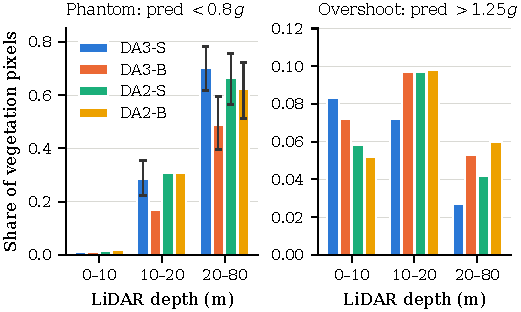
\includegraphics[width=\columnwidth]{fig_distance.pdf}
\caption{Phantom rate ($\pred<0.8\,\gt$) and overshoot rate ($\pred>1.25\,\gt$) on vegetation by LiDAR distance, primary alignment. Error bars are 95\% block-bootstrap intervals where we computed them.}
\label{fig:dist}
\end{figure}

One objection is that this is just an artefact of scale-only alignment and a shift term would absorb it. We checked this on grass with every estimator. A shift in inverse depth does help: far-grass (20--80\,m) \absrel{} for DA3-S goes from 0.313 with \texttt{median} to 0.287 with \texttt{ls} and 0.253 with Huber, and the far-grass phantom rate from 0.72 to 0.58 and 0.50. But even the best case, DA3-B with Huber (far-grass \absrel{} 0.210), still has 43\% far-grass phantoms, and the near/far asymmetry is there under every estimator. No per-image scale or scale-and-shift fit removes the compression. We think this is the real-data version of the phantom obstacle problem in~\cite{offroadnav}: a field of far grass placed 20--30\% too close looks like an obstacle to a planner. Two caveats. LiDAR returns in tall grass can come from the grass top or the ground, so the far-grass ground truth is itself uncertain. And the far-grass numbers move by about 13\% under the sensitivity calibration (Sec.~\ref{sec:sens}).

\subsection{Label source}\label{sec:labels}
The terrain groups come from the LiDAR point labels. On the 2{,}074 annotated test frames we also computed the groups from the 2D image annotations sampled at the LiDAR pixels. The model ranking does not change and the grass and vegetation numbers move by at most 0.02. Trees/bushes and ground do depend on the label source (for DA3-S, trees/bushes \absrel{} is 0.296 with LiDAR labels and 0.229 with image labels; ground is 0.228 and 0.470). Image labels inherit the calibration offset, and the two sources disagree on grass versus bush: where LiDAR says grass, the image annotation says bush 4--14\% of the time, and in 00002 frames 1215--1277 a whole field is grass in one and bush in the other. So we treat vegetation (grass plus trees/bushes) as the reliable group and the per-class ground numbers with care.

\subsection{Confidence quality}\label{sec:conf}
Table~\ref{tab:conf} and Fig.~\ref{fig:spars} look at the DA3 confidence as a detector of its own errors. The per-image AUROC for pixels with \absrel{} $>0.25$ is 0.882 \ci{0.853}{0.901} for DA3-S and 0.894 for DA3-B with \texttt{median}, and 0.90--0.92 with the two-parameter alignments. AUSE is 0.021--0.033 and AURG is 0.059--0.068. Paired, DA3-B ranks errors slightly better (AUROC $+0.012$ \ci{0.002}{0.021} with \texttt{median}) but gains slightly less from filtering (AURG $-0.004$ \ci{-0.009}{-0.000}). The numbers are stable across alignments and both calibrations (AUROC 0.879 with the sensitivity ground truth). We only evaluate the ranking. Nothing here says the confidence is calibrated.

\begin{table}[!t]
\caption{Confidence quality of DA3 on test. AUROC for \absrel{} $>0.25$; AUSE and AURG from sparsification. 95\% intervals.}
\label{tab:conf}
\centering
\footnotesize
\setlength{\tabcolsep}{3pt}
\begin{tabular}{llccc}
\toprule
Model & Align. & AUROC $\uparrow$ & AUSE $\downarrow$ & AURG $\uparrow$ \\
\midrule
DA3-S & median & 0.882 \ci{.853}{.901} & 0.033 \ci{.027}{.041} & 0.064 \ci{.051}{.080} \\
DA3-S & ls     & 0.906 \ci{.895}{.917} & 0.022 \ci{.020}{.023} & 0.062 \ci{.050}{.078} \\
DA3-S & huber  & 0.900 \ci{.889}{.911} & 0.023 \ci{.021}{.024} & 0.068 \ci{.053}{.089} \\
DA3-B & median & 0.894 \ci{.859}{.913} & 0.032 \ci{.025}{.045} & 0.060 \ci{.045}{.076} \\
DA3-B & ls     & 0.916 \ci{.906}{.924} & 0.021 \ci{.019}{.022} & 0.059 \ci{.048}{.074} \\
DA3-B & huber  & 0.909 \ci{.900}{.919} & 0.022 \ci{.020}{.023} & 0.065 \ci{.051}{.084} \\
\bottomrule
\end{tabular}
\end{table}

\begin{figure}[!t]
\centering
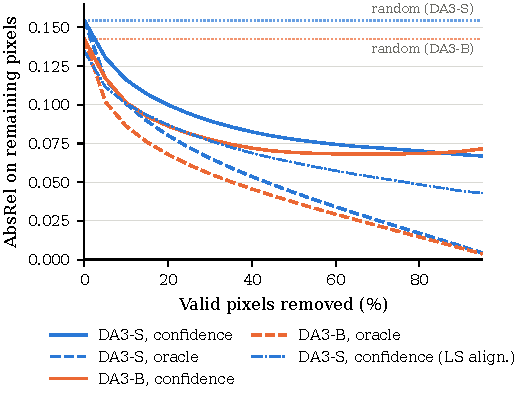
\includegraphics[width=\columnwidth]{fig_sparsification.pdf}
\caption{Sparsification curves on test: mean \absrel{} after removing the lowest-confidence share of valid pixels (solid) against removal by true error (oracle, dashed), scale-only alignment. Dotted lines are random removal. The dash-dotted curve is DA3-S with scale-and-shift (\texttt{ls}) alignment.}
\label{fig:spars}
\end{figure}

The sparsification curves show one more thing. With scale-only alignment the confidence curve flattens out after about 50--60\% removal at roughly 0.07 \absrel{}, while with scale-and-shift it keeps going down to about 0.043. So after scale-only alignment there is a leftover error that the confidence cannot rank. This fits a global distance-dependent distortion (Sec.~\ref{sec:dist}) better than per-pixel noise, but we have not tested this.

\subsection{Filtering at equal budgets}\label{sec:filter}
Table~\ref{tab:filter} and Fig.~\ref{fig:filter} give the main filtering result. Removing the 20\% of valid pixels with the lowest DA3-S confidence brings \absrel{} from 0.155 down to 0.100. Removing the 20\% with the highest Sobel magnitude leaves it at 0.151. The paired difference is $-0.052$ \ci{-0.065}{-0.039}, and it grows with the budget to $-0.095$ at 50\%. The phantom rate behaves the same way: at 20\%, confidence filtering cuts it from 0.106 to 0.049 while Sobel filtering leaves 0.110, and at 50\% confidence removes nearly all phantoms (0.010) while Sobel removal actually increases them (0.126). DA3-B gives the same picture, and so do the \texttt{ls} and \texttt{huber} alignments.

The Sobel signal is close to random. Compared with random removal, Sobel-ranked removal gains only $-0.006$ at 10\% and $-0.003$ at 20\% (interval touching zero), nothing at 30\%, and is worse than random at 50\% ($+0.018$ \ci{0.008}{0.026} for DA3-S, $+0.011$ for DA2-S). Confidence-ranked removal gains $-0.038$ to $-0.077$. The reason seems simple. The edge mask removes pixels next to depth discontinuities, and those pixels do have high error (Table~\ref{tab:headline}), but the edge band is only about 4\% of the LiDAR-valid pixels. Most of the error is in smooth far vegetation (Sec.~\ref{sec:dist}), which has no gradient to detect.

\begin{table}[!t]
\caption{\absrel{} on the remaining valid pixels after removing a fixed share, primary alignment. Random removal gives the unfiltered value (0.155 / 0.142 / 0.165 / 0.169) in expectation. Last column: paired confidence$-$Sobel difference with 95\% interval.}
\label{tab:filter}
\centering
\scriptsize
\setlength{\tabcolsep}{3.5pt}
\begin{tabular}{lc ccc c}
\toprule
Model & Budget & Sobel & Conf. & Random & Conf.$-$Sobel \\
\midrule
DA3-S & 10\% & 0.148 & 0.116 & 0.155 & $-0.032$ \ci{$-$.042}{$-$.023} \\
DA3-S & 20\% & 0.151 & \textbf{0.100} & 0.155 & $\mathbf{-0.052}$ \ci{$-$.065}{$-$.039} \\
DA3-S & 30\% & 0.157 & 0.090 & 0.155 & $-0.067$ \ci{$-$.083}{$-$.049} \\
DA3-S & 50\% & 0.173 & 0.078 & 0.155 & $-0.095$ \ci{$-$.118}{$-$.070} \\
\addlinespace[2pt]
DA3-B & 10\% & 0.136 & 0.101 & 0.142 & $-0.034$ \ci{$-$.044}{$-$.025} \\
DA3-B & 20\% & 0.139 & 0.086 & 0.142 & $-0.052$ \ci{$-$.066}{$-$.040} \\
DA3-B & 30\% & 0.144 & 0.078 & 0.142 & $-0.067$ \ci{$-$.084}{$-$.051} \\
DA3-B & 50\% & 0.163 & 0.069 & 0.142 & $-0.094$ \ci{$-$.117}{$-$.070} \\
\addlinespace[2pt]
DA2-S & 10/20/30/50\% & \multicolumn{3}{l}{Sobel: .149 / .152 / .158 / .176} & -- \\
DA2-B & 10/20/30/50\% & \multicolumn{3}{l}{Sobel: .148 / .150 / .155 / .172} & -- \\
\bottomrule
\end{tabular}
\end{table}

\begin{figure}[!t]
\centering
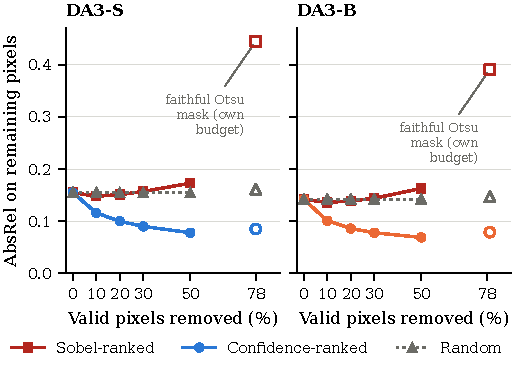
\includegraphics[width=\columnwidth]{fig_filtering.pdf}
\caption{\absrel{} on the remaining valid pixels against the share removed, for Sobel-ranked, confidence-ranked and random removal (primary alignment). Hollow markers: the faithful Otsu mask of~\cite{offroadnav} at thickness 5, which removes about 78\% of valid pixels, with confidence and random removal matched to that budget. The Otsu point is averaged over the 742 (DA3-S) or 830 (DA3-B) images where every filter left at least 50 pixels.}
\label{fig:filter}
\end{figure}

\subsection{The faithful edge mask}\label{sec:otsu}
Table~\ref{tab:otsu} applies the Otsu mask exactly as shipped, at thickness 5. On RELLIS-3D at $504\times322$ it removes about half of the whole image but 78--79\% of the LiDAR-valid pixels for DA3 (51--57\% for DA2), because the valid pixels are in the textured lower half of the frame and Otsu mostly separates the smooth sky from everything else. Worse, the pixels it keeps have much higher error than average: \absrel{} 0.39--0.45 for DA3 against 0.155 unfiltered. Removing the same number of valid pixels by lowest confidence gives 0.085 instead (paired difference $-0.36$ \ci{-0.52}{-0.22} for DA3-S). Thickness 3 and 9 give the same picture. A likely reason is that the low-gradient areas are mostly far vegetation, the worst region in Sec.~\ref{sec:dist}, but we have not tested that. These numbers are for RELLIS-like scenes at our resolution and our re-implementation. They do not show that the stack of~\cite{offroadnav} works badly in its own setting; its camera resolution is not in the repository and its default detector is Canny.

\begin{table}[!t]
\caption{The Otsu edge mask as shipped (thickness 5): share of valid pixels and of the whole image removed, and \absrel{} on the kept pixels against confidence removal matched to the same valid-pixel count (conf\_valid) or whole-image share (conf\_all).}
\label{tab:otsu}
\centering
\footnotesize
\setlength{\tabcolsep}{3.5pt}
\begin{tabular}{l cc ccc c}
\toprule
 & \multicolumn{2}{c}{Removed} & \multicolumn{3}{c}{\absrel{} at same budget} & \\
\cmidrule(lr){2-3}\cmidrule(lr){4-6}
Model & valid & image & Sobel & conf\_valid & conf\_all & random \\
\midrule
DA3-S & 0.779 & 0.490 & 0.445\n{742} & 0.085 & 0.119 & 0.161 \\
DA3-B & 0.792 & 0.488 & 0.391 & 0.079 & 0.111 & 0.147 \\
DA2-S & 0.569 & 0.349 & 0.328 & -- & -- & 0.168 \\
DA2-B & 0.505 & 0.315 & 0.302 & -- & -- & 0.174 \\
\bottomrule
\end{tabular}
\end{table}

\subsection{Calibration sensitivity}\label{sec:sens}
We recomputed everything against the sensitivity ground truth from Sec.~\ref{sec:calib}. Overall \absrel{} barely moves (DA3-S 0.155 to 0.155, DA2-S 0.165 to 0.170), and neither do the model ranking, the confidence result (DA3-S AUROC 0.882 to 0.879), the filtering result (confidence$-$Sobel at 20\%: $-0.052$ to $-0.050$) or the paired DA2-S--DA3-S gap with \texttt{ls} ($+0.030$ to $+0.033$ overall, $+0.108$ to $+0.109$ on depth edges). What does move are DA3's absolute edge and far-grass numbers under scale-only alignment: for DA3-S, edge \absrel{} goes from 0.343 to 0.322 ($-6$\%), far-grass \absrel{} from 0.313 to 0.354 ($+13$\%) and the phantom rate from 0.106 to 0.119 ($+12$\%). DA2 moves by at most 3\%. So DA3's edge and far-grass values carry about $\pm10$\% calibration uncertainty, while every comparison between models is robust to it.

\section{Limitations}
All five sequences come from one campus recorded over two days, so the test sequence is unseen but the place is not, and we have no second dataset. The calibration offset (Sec.~\ref{sec:calib}) has an unknown cause and puts about $\pm10$\% uncertainty on DA3's edge and far-grass numbers. Per-image alignment uses LiDAR that a robot would not have. LiDAR returns in tall grass may hit the grass top or the ground, so the grass ground truth is itself uncertain, and the grass/bush labels disagree between sources. The edge band is defined on sparse LiDAR with row $\pm1$, so horizontal edges between rings are missed. Ground and other have only 2--4 points per test image, so their numbers rest on few images. The edge-mask comparison is our re-implementation at our resolution, not the full pipeline of~\cite{offroadnav}, and we did not run any closed-loop navigation test. Finally, we only evaluate the ranking of the confidence, and confidence cannot help where tall grass really is an obstacle.

\section{Conclusion}
On real off-road LiDAR, zero-shot DA3-Small is more accurate than zero-shot DA2 when both are aligned the same way, by 0.030 \absrel{} overall and 0.108 on depth edges, while on grass the two families are about equal. All four models compress far range: beyond 20\,m, half to two thirds of vegetation pixels are placed closer than 0.8 times their LiDAR depth, no per-image alignment removes this, and DA3-Base is the least affected. The DA3 confidence ranks its own errors well (AUROC 0.88--0.92), and at the same pixel budget it removes much more error than the Sobel edge signal used by an open-source off-road stack, which is barely better than random at small budgets and worse than random at 50\%. The stack's Otsu mask, applied as shipped, throws away most LiDAR-covered pixels and keeps the worst ones. These conclusions hold under least-squares and Huber alignment, both calibrations and both label sources.

For someone putting a zero-shot depth model on an off-road robot, the practical message is that an edge mask only addresses a small part of the error, that DA3's confidence is a much better per-pixel filter, and that even then a systematic far-range compression is left that no filter can fix. Whether a small fine-tune on off-road LiDAR removes it is the next question, and the numbers here are the baseline for that. The projection and evaluation code is released under Apache~2.0; a full test run takes about seven minutes on a laptop GPU. RELLIS-3D is used under CC~BY-NC-SA~3.0.

\begin{thebibliography}{00}
\bibitem{da1} L. Yang, B. Kang, Z. Huang, X. Xu, J. Feng, and H. Zhao, ``Depth Anything: Unleashing the power of large-scale unlabeled data,'' in \emph{Proc. IEEE/CVF Conf. Comput. Vis. Pattern Recognit. (CVPR)}, 2024.
\bibitem{da2} L. Yang, B. Kang, Z. Huang, Z. Zhao, X. Xu, J. Feng, and H. Zhao, ``Depth Anything V2,'' in \emph{Adv. Neural Inf. Process. Syst. (NeurIPS)}, 2024, arXiv:2406.09414.
\bibitem{da3} H. Lin, S. Chen, J. Liew, D. Y. Chen, Z. Li, G. Shi, J. Feng, and B. Kang, ``Depth Anything 3: Recovering the visual space from any views,'' arXiv:2511.10647, Nov. 2025.
\bibitem{offroadnav} R. Marsal, Q. Picard, A. Poir\'e, S. Kerbourc'h, T. Toralba, C. Yver, A. Chapoutot, and D. Filliat, ``An open-source LiDAR and monocular off-road autonomous navigation stack,'' arXiv:2604.03096, Apr. 2026. Code: \url{https://github.com/LARIAD/Offroad-Nav}.
\bibitem{rellis} P. Jiang, P. Osteen, M. Wigness, and S. Saripalli, ``RELLIS-3D dataset: Data, benchmarks and analysis,'' in \emph{Proc. IEEE Int. Conf. Robot. Autom. (ICRA)}, 2021, arXiv:2011.12954.
\bibitem{hillemann} M. Hillemann, R. Langend\"orfer, S. Landgraf, and M. Ulrich, ``Uncertainty quality of VGGT: An analysis on the DTU benchmark dataset,'' arXiv:2606.16479, Jun. 2026.
\bibitem{deng} N. N. Deng, Q. Cheng, N. Zeller, and D. Cremers, ``A calibration audit of confidence in feed-forward 3D reconstruction models,'' arXiv:2608.29705, Aug. 2026.
\bibitem{trust3r} Z. Zhu, W. Zhao, N. Chen, C. Tian, and Z. Fan, ``Trust it or not: Evidential uncertainty for feed-forward 3D reconstruction with Trust3R,'' arXiv:2605.19539, May 2026.
\bibitem{revar3r} S. Mahdi, F. B. Salim, R. B. Rabbani, and A. N. Zereen, ``ReVar3R: Gauge-aware perturbation uncertainty for feed-forward 3D reconstruction,'' arXiv:2610.07883, Oct. 2026.
\bibitem{landgraf} S. Landgraf, R. Qin, and M. Ulrich, ``A critical synthesis of uncertainty quantification and foundation models in monocular depth estimation,'' arXiv:2501.08188, Jan. 2025.
\bibitem{ilg} E. Ilg, \"O. \c{C}i\c{c}ek, S. Galesso, A. Klein, O. Makansi, F. Hutter, and T. Brox, ``Uncertainty estimates and multi-hypotheses networks for optical flow,'' in \emph{Proc. Eur. Conf. Comput. Vis. (ECCV)}, 2018.
\bibitem{underwater} Z. Cai and C. Metzler, ``Underwater monocular metric depth estimation: Real-world benchmarks and synthetic fine-tuning with vision foundation models,'' arXiv:2507.02148, Jul. 2025.
\bibitem{endo} B. Li, B. Liu, X. Yao, J. Yue, and F. Zhou, ``Advancing Depth Anything model for unsupervised monocular depth estimation in endoscopy,'' arXiv:2409.07723, Sep. 2024.
\bibitem{canopy} D. R. Cambrin, I. Corley, and P. Garza, ``Depth Any Canopy: Leveraging depth foundation models for canopy height estimation,'' arXiv:2408.04523, Aug. 2024.
\bibitem{huber} P. J. Huber, \emph{Robust Statistics}. New York, NY, USA: Wiley, 1981.
\bibitem{otsu} N. Otsu, ``A threshold selection method from gray-level histograms,'' \emph{IEEE Trans. Syst., Man, Cybern.}, vol. 9, no. 1, pp. 62--66, Jan. 1979.
\end{thebibliography}

\end{document}
